\section{کتابخوان}

\subsection{اهداف آزمایش}
\begin{itemize}
    \item آشنایی با پروتکل ارتباط سریال \lr{I2C}
    \item کار با حافظه‌ی \lr{EEPROM} بیرونی و نحوه‌ی خواندن از آن
\end{itemize}
\subsection{قطعات مورد نیاز}
\begin{itemize}
    \item \lr{Arduino Uno}
    \item صفحه نمایش \lr{LCD}
    \item پتانسیومتر ۱ کیلواهم \lr{B1K}
    \item مقاومت ۲۲۰ اهم
    \item \lr{EEPROM (AT24C16)}
    \item کلید \lr{Switch}
    \item مقاومت ۱۰ هزار اهم
\end{itemize}
\subsection{مقدمه}
در این آزمایش میخواهیم با نحوه کار با حافظه 
\lr{EEPROM}
آشنا شویم و از آن برای نمایش دادن یک کتاب که متن آن درون این حافظه‌ی بیرونی ذخیره شده استفاده کنیم. برای نمایش دادن خط به خط کتاب بر روی
\lr{LCD}
با استفاده از ۲ کلیدی که در مدار قرار می‌دهیم به خط قبلی یا خط بعدی کتاب می‌رویم.

\newline
\begin{nas}حافظه \lr{EEPROM}\end{nas}
\newline

در بسیاری از برنامه ها ما نیاز داریم که اطلاعاتی را ذخیره کنیم تا پس از اجرای مجدد برنامه از آنها استفاده کنیم. همچنین اطلاعاتی که حجم زیادی دارند را نمی‌توان در حافظه‌ی خود برد ذخیره کرد و نیاز داریم که یک حافظه بیرونی برای ذخیره این اطلاعات داشته باشیم که پس از متوقف کردن برنامه نیز اطلاعات در آن ذخیره بمانند. همچنین در دنیای میکروکنترلر ها یکی از اصلی ترین مسائلی که قیمت میکروکنترلر های مختلف را متفاوت می‌کند میزان حافظه‌ی آنهاست و یکی از راه هایی که می‌توان قیمت تمام شده‌ی یک محصول دارای یک سیستم نهفته را کمتر کرد استفاده از میکروکنترلری با حافظه‌ی کمتر و وصل کردن یک حافظه‌ی بیرونی به آن است.
 به همین دلیل ما به \lr{EEPROM} ها نیاز داریم.
\newline
در یک دسته‌بندی می‌توان \lr{EEPROM} ها را به دو نوع درونی و بیرونی دسته‌بندی کرد. حافظه‌های درونی در کنار پردازنده بر روی همان مدار مجتمع قرار می‌گیرند و نیازی به استفاده از پایه های آدرس ندارند. همچنین به دلیل حضور در یک مدار مجتمع اتصال بهتری میان آن‌ها و میکروکنترلر برقرار است و سرعت آن‌ها بیشتر است. بورد \lr{Arduino Uno} نیز یک حافظه ی \lr{EEPROM} درونی به اندازه ۱ کیلوبایت دارد که در این آزمایش مورد توجه ما نیست.
\newline
 گونه‌ای دیگر از 
 \lr{EEPROM}
 ها بیرونی هستند که بر روی یک 
 \lr{IC}
 جداگانه قرار میگیرند. برای ارتباط با این حافظه‌ها اکثرا از پروتکل‌های ارتباط سریال استفاده میشود. حافظه 
 \lr{AT24C16}
 نیز که در این آزمایش به کار برده میشود، پروتکل سریال 
 \lr{TWI}
 را به کار میگیرد. به این صورت که در این پروتکل حافظه‌ها همان برده‌ها 
 \lr{(Slaves)}
 هستند و برد کنترلر نیز سرپرست  
 \lr{(Master)}
 است. در این دسته گاهی برای اینکه بتوان چند حافظه را بر روی یک باس کنترل کرد (چند برده داشت) از پایه‌های آدرس استفاده میشود. این آدرس به صورت سخت‌افزاری پیکربندی میشود 
 \lr{(Hard-Wired)}
 .
\newline

\lr{AT24C16}
از پروتکل 
\lr{TWI}
یا همان \lr{I2C} استفاده می‌کند و مطابق چیزی که از این پروتکل می‌دانیم باید ۷ بیت آدرس داشته باشد. چهار بیت پر ارزش آدرس آن مقدار ثابت \lr{0b1010} است و سه بیت کم ارزش آن را پایه های
\lr{A0} تا \lr{A3}
مشخص می‌کند. البته این پایه ها در واقعیت ممکن است استفاده بشوند یا نشوند. در واقع چیپ حافظه‌ی \lr{AT24C16} از این پین ها استفاده نمی‌کند و همواره سه بیت کم ارزش آدرس آن صفر است و چیپ \lr{AT24C08} نیز فقط از پین \lr{A2} استفاده می‌کند و دو پین دیگر همواره صفر هستند. همیشه برای اینگونه فهمیدن جزئیات کار با قطعات الکترونیکی به دیتاشیت قطعه مراجعه کنید.
\newline
همچنین 
\lr{EEPROM}
پایه ای به نام 
\lr{WP}
دارد که مخفف 
\lr{Write Protection}
است که اگر مقدار منطقی آن برابر یک باشد و به عبارتی به آن ولتاژ وارد شود، فعال میشود و امکان نوشتن روی 
\lr{EEPROM}
دیگر وجود ندارد.
دو تصویر از پایه های 
\lr{AT24C16}
و کارکرد هرکدام از آن‌ها نمایش داده شده است.

\newline
\begin{figure}[h]
    \centering
    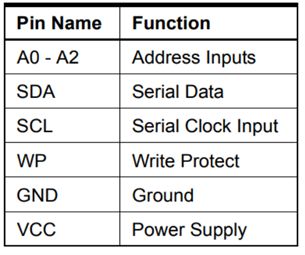
\includegraphics[width=8cm]{eeprom-pindesc.png}
    \caption{کارکرد پین های حافظه}
    \label{fig:eeprom-pindesc}
\end{figure}

\begin{figure}[h]
    \centering
    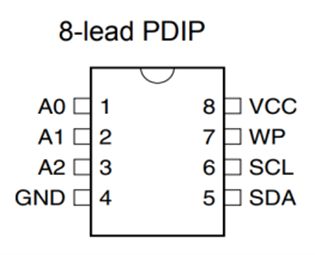
\includegraphics[width=8cm]{eeprom-pinout.png}
    \caption{دیاگرام پین های حافظه}
    \label{fig:eeprom-pinout}
\end{figure}
\newline

\begin{nas} کار با کتابخانه \lr{TWI} در \lr{Arduino} \end{nas}
\newline

کتابخانه 
\lr{wire.h}
یکی از کتابخانه‌های استاندارد آردوینو است که نیازی به نصب آن نیست. این کتابخانه توابع لازم برای کار با پروتکل \lr{TWI} را فراهم میکند. برخی از توابع این کتابخانه به شرح زیر است:
\begin{itemize}
    \item \lr{begin()}
    \item \lr{setClock()}
    \item \lr{beginTransmission()}
    \item \lr{write()}
    \item \lr{endTransmission()}
    \item \lr{requestFrom()}
    \item \lr{available()}
    \item \lr{read()}
\end{itemize}

\textcolor{red}{\begin{nas}سوال: \end{nas}}
هر یک از توابع بالا را در مستندات کتابخانه بررسی کنید و ورودی ها، خروجی ها و عملکرد آنها را توضیح دهید.
\pagebreak
\newline

\begin{nas}چگونگی خواندن و نوشتن بر روی حافظه‌ی \lr{EEPROM}\end{nas}
\newline
الگوریتم خواندن به صورت زیر است:
\begin{enumerate}
    \item شروع ارتباط با دستگاهی که آدرس \lr{I2C} آن آدرس حافظه‌ی ما است.
    \item نوشتن یک بایت آدرس حافظه‌ای که می‌خواهیم بخوانیم.
    \item پایان ارتباط.
    \item درخواست تعداد بایت دلخواه از دستگاهی که آدرس \lr{I2C} آن آدرس حافظه‌ی ما است.
    \item به اندازه‌ی بایت هایی که درخواست کردیم داده می‌خوانیم.
\end{enumerate}

الگوریتم نوشتن به صورت زیر است:
\begin{enumerate}
    \item شروع ارتباط با دستگاهی که آدرس \lr{I2C} آن آدرس حافظه‌ی ما است.
    \item نوشتن یک بایت آدرس حافظه‌ای که می‌خواهیم در آن بنویسیم.
    \item نوشتن بایت هایی که می‌خواهیم بنویسیم.
    \item پایان ارتباط.
\end{enumerate}

\subsection{شرح آزمایش}

\paragraph{
ابتدا اتصالات مربوط به حافظه را کامل کنید. مشخصا پایه های \lr{VCC} و \lr{GND} باید به مثبت و زمین وصل شوند. همه پایه های آدرس و پایه \lr{WP} را نیز به زمین وصل کنید. پایه های کلاک و دیتا را باید به پایه های مخصوص کلاک و دیتای پروتکل \lr{I2C} آردوینو وصل کنید. نقشه‌ای از پین های آردوینو در قسمت «راهنمای پین‌های آردوینو» آمده که می‌توانید از آن استفاده کنید.
}

\paragraph{
یک چیپ حافظه به شما داده می‌شود که از قبل روی آن یک متن ذخیره شده. شما باید ۱۶ کاراکتر از این متن را بخوانید و روی صفحه‌نمایش نمایش دهید. همچنین دو کلید داشته باشید که با فشردن این دو کلید دستگاه شما ۱۶ کاراکتر بعدی یا قبلی متن را بخواند و نمایش دهد. 
توجه کنید نیازی به نوشتن چیزی بر روی حافظه نیست و این کار از قبل برای شما انجام شده است.
}